\documentclass[../../main.tex]{subfiles}
    
    \lstset{basicstyle=\small,
      showstringspaces=false,
      commentstyle=\color{black},
      keywordstyle=\color{blue}
    }

    \graphicspath{{images/}{../../images/Objekterkennung/}}

    \begin{document}
    \subsection{Objekterkennung}
    In der Anforderungsliste werden verschiedene Objekterkennungen gefordert. Signal inklusive Nummer,
    Würfelerkennung, Lichtraumprofilerkennung so wie Spurrichtungserkennung sollen umgesetzt werden. Dafür 
    kommen verschiedene Konzepte in Frage. In diesem Kapitel soll diese verschiedene Konzepte analysiert 
    werden.\\

    \textbf{Auswahl interdisziplin Konzepte}\\
    Die Objekterkennung kann je nach Problemstellung mit unterschiedlichen Disziplinen (Mechanik,
    Elektrotechnik und Informatik) gelöst werden. In der Tabelle \ref{tab:obj_disziplin} wird
    aufgelistet welche Problemstellung mit welcher Disziplin gelöst werden kann.
    %Tabelle mit DisziplinKonzepte
    \begin{flushleft}
        \begin{table}[h]
        \begin{tabular}{ | l | p{11cm} |}
        \hline
        \textbf{Disziplin} & \textbf{Konzepte} \\ \hline
        Mechanik & \begin{itemize}
                        \item Spurrichtungserkennung
                    \end{itemize} \\ \hline
        Elektrotechnik & \begin{itemize}
                             \item Würfelerkennung
                             \item Spurrichtungserkennung
                             \item Lichtraumprofilerkennung
                         \end{itemize} \\ \hline
        Informatik &  \begin{itemize}
                        \item Würfelerkennung
                        \item Spurrichtungserkennung
                        \item Lichtraumprofilerkennung
                        \item Signalerkennung
                      \end{itemize} \\ \hline
        \end{tabular}
        \caption{Disziplinentabelle}
        \label{tab:obj_disziplin}
    \end{table}
    \end{flushleft}

    Im Folgenden werden die möglichen Konzepte pro Problemstellung analysiert. Für die Disziplin Informatik
    wird immer das Konzept «Kamera» verwendet.

    \subsubsection{Würfelerkennung}
    Die Problemstellung «Würfelerkennung» kann entweder mit der Disziplin Elektrotechnik oder Informatik
    gelöst werden. Bei der «Würfelerkennung» muss im Startbereich einen Holzwürfel erkennt,
    Position des Würfels ermittelt und diesen mittels Kran auf den Zug geladen werden 
    (siehe Abbildung \ref{fig:wurfelerkennung}).

    \begin{figure}[H] %Ablaufdiagramm Vision
        \centering
        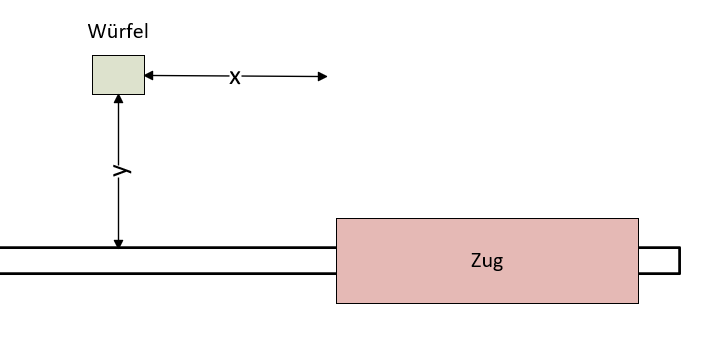
\includegraphics[width=0.7\textwidth]{wurfelerkennung.png}
        \caption{Positionsbestimmung des Würfels}
        \label{fig:wurfelerkennung}
    \end{figure}

    \textbf{Elektrotechnik: }
    Mittels Ultraschallsensor kann der Würfel erkennt und seine Position ermittel werden. Der Ultraschallsensor
    wird seitlich am Zug positioniert und misst kontinuierlich den Abstand. Sobald ein Gegenstand mit der Form und
    Grösse des Würfels erkennt wird hält der Zug und der Kran kann sich anhand des ermittelten Abstandes 
    positionieren.
    \begin{figure}[H] %Ablaufdiagramm Vision
        \centering
        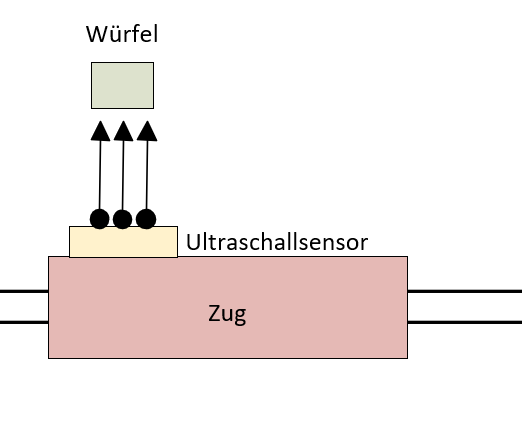
\includegraphics[width=0.4\textwidth]{Ultraschallsensor.png}
        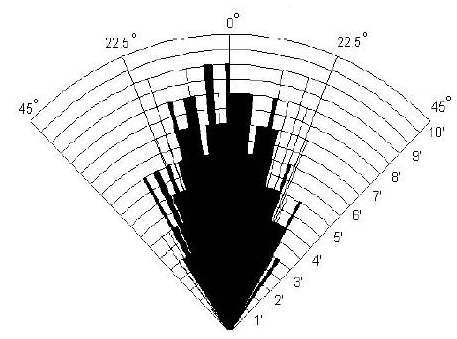
\includegraphics[width=0.4\textwidth]{Ultraschallsensor_angle.png}
        \caption{Objekterkennung und Positionsbestimmung mittels Ultraschallsensor}
        \label{fig:wurfel_ultraschall}
    \end{figure}

    \begin{flushleft}
        \begin{table}[h]
        \begin{tabular}{ | l | p{11cm} |}
        \hline
        \textbf{Problemstellung} & Würfelerkennung \\ \hline
        \textbf{Disziplin} & Elektrotechnik \\ \hline
        \textbf{Lösungskonzept} & Objekterkennung und Positionsbestimmung mittels Ultraschallsensor \\ \hline
        \textbf{Komponente} & Ultraschallsensor HC-SR04 \\ \hline
        \textbf{Bewertung} &  \begin{itemize}
                                \item[+] Schnelligkeit
                                \item[+] Einfachheit
                                \item[+] geringe Kosten 
                                \item[-] weitere Auswertungslogik nötig
                                \item[-] Abstand Zug <=> Würfel limitiert   
                              \end{itemize} \\ \hline
        \end{tabular}
        \caption{Konzeptbeurteilung: Würfelerkennung mittels Ultraschallsensor}
        \label{tab:konzept_wurfel_ultraschall}
    \end{table}
    \end{flushleft}

    \vspace{0.5cm}
    \textbf{Informatik: }
    Eine weitere Methode den Würfel zu erkennen ist die Objekterkennung mittels Kamera. Hier wird die Kamera am Zug
    befestigt und mittels Software den Würfel gesucht. Um die Position des Würfels im Raum zu ermitteln, wird eine 
    Stereokamera gebraucht. Damit lassen sich Tiefeninformationen und somit den Abstand vom Zug zum Würfel ermitteln.\\
    
    \begin{figure}[H] %Ablaufdiagramm Vision
        \centering
        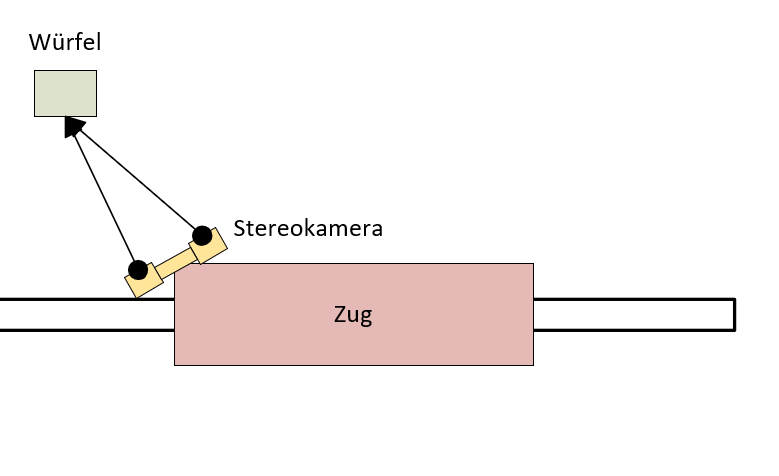
\includegraphics[width=0.4\textwidth]{wurfel_Stereokamera.png}
        \caption{Objekterkennung und Positionsbestimmung mittels Stereokamera}
    \end{figure}

    \begin{flushleft}
        \begin{table}[H]
        \begin{tabular}{ | l | p{11cm} |}
        \hline
        \textbf{Problemstellung} & Würfelerkennung \\ \hline
        \textbf{Disziplin} & Informatik \\ \hline
        \textbf{Lösungskonzept} & Objekterkennung und Positionsbestimmung mittels Stereokamera \\ \hline
        \textbf{Komponente} & Intel RealSense \\ \hline
        \textbf{Bewertung} &  \begin{itemize}
                                \item[+] Hoher Abstandsrange
                                \item[+] Zuverlässigkeit
                                \item[-] hohe Kosten 
                                \item[-] Komplexität
                                \item[-] Schnelligkeit   
                              \end{itemize} \\ \hline
        \end{tabular}
        \caption{Konzeptbeurteilung: Würfelerkennung mittels Stereokamera}
        \label{tab:konzept_wurfel_Stereokamera}
    \end{table}
    \end{flushleft}


    \subsubsection{Spurrichtungserkennung}
    Bei der «Spurrichtungserkennung» wird gebraucht um so schnell wie möglich mit dem Zug um die Kurven zu fahren.
    Mit der «Spurrichtungserkennung» muss der Radius der zu fahrenden Kurve so früh wie möglich erkannt werden, damit
    der Zug auf die richtige Geschwindigkeit gebracht werden kann. Für diese Problemstellung gibt es eine mechatronische-
    und eine Informatik Lösung.\\

    \textbf{Mechatronik: }
    Bei der mechatronischen Lösung wird vor dem Zug ein kleiner «Sensor- Wagen» gespannt, welcher mittels einer Achse
    mit dem Zug befestigt ist. Sobald der kleine und leichte «Sensor- Wagen» in die Kurve einfahrt, wird die Achse gedreht
    und somit kann der Radius der Kurve ermittelt werden.\\
    \begin{figure}[H] %Ablaufdiagramm Vision
        \centering
        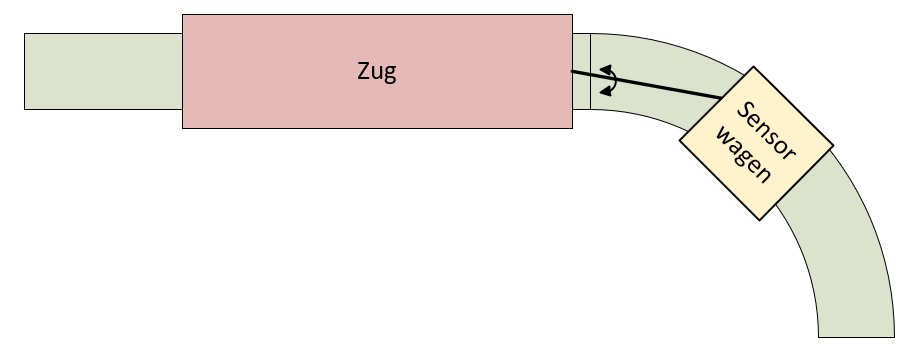
\includegraphics[width=0.8\textwidth]{spurrichtung_mechatronik.png}
        \caption{Spurrichtungserkennung mittels «Sensor- Wagen»}
    \end{figure}

    \begin{flushleft}
        \begin{table}[H]
        \begin{tabular}{ | l | p{11cm} |}
        \hline
        \textbf{Problemstellung} & Spurrichtungserkennung \\ \hline
        \textbf{Disziplin} & Mechatronik \\ \hline
        \textbf{Lösungskonzept} & Erkennung mittels «Sensor- Wagen» \\ \hline
        \textbf{Komponente} & Eigenbau und (Winkelsensor) \\ \hline
        \textbf{Bewertung} &  \begin{itemize}
                                \item[+] Einfachheit
                                \item[+] kostengünstig
                                \item[-] Zuverlässigkeit
                                \item[-] Auflösung   
                              \end{itemize} \\ \hline
        \end{tabular}
        \caption{Konzeptbeurteilung: Würfelerkennung mittels Stereokamera}
        \label{tab:konzept_wurfel_Stereokamera}
    \end{table}
    \end{flushleft}

    \vspace{0.5cm}
    \textbf{Informatik: }
    Eine zweite mögliche Lösung wäre der Einsatz einer Kamera. Die Kamera müsste im unteren Teil des Zuges befestigt
    werden, damit der Spurverlauf gut analysiert werden kann. Wenn die Spur nun die Richtung ändert kann man dies 
    anhand der Kamera feststellen.\\

    \begin{figure}[H] %Ablaufdiagramm Vision
        \centering
        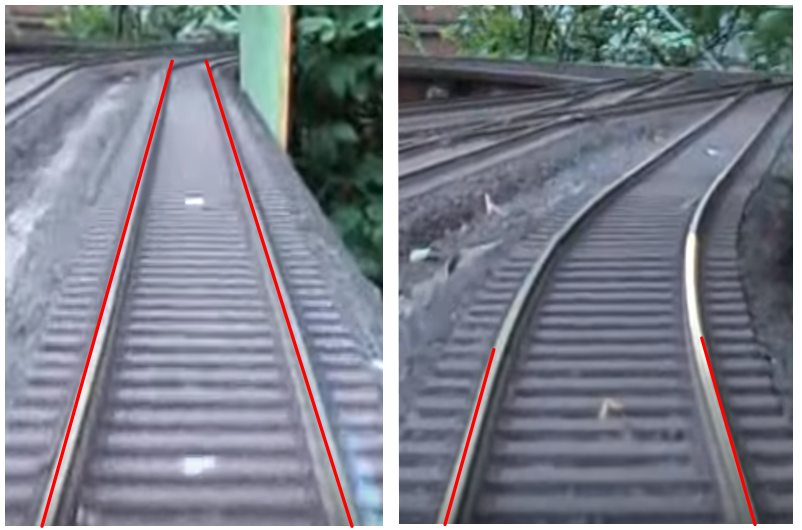
\includegraphics[width=0.8\textwidth]{spurrichtung_Kamera.png}
        \caption{Spurrichtungserkennung mittels Kamera}
    \end{figure}

    \begin{flushleft}
        \begin{table}[H]
        \begin{tabular}{ | l | p{11cm} |}
        \hline
        \textbf{Problemstellung} & Spurrichtungserkennung \\ \hline
        \textbf{Disziplin} & Informatik \\ \hline
        \textbf{Lösungskonzept} & Erkennung mittels Kamera \\ \hline
        \textbf{Komponente} & OV5647 \\ \hline
        \textbf{Bewertung} &  \begin{itemize}
                                \item[+] Einfachheit (Hardware)
                                \item[+] kostengünstig
                                \item[-] Zuverlässigkeit
                                \item[-] Komplexität (Software)   
                              \end{itemize} \\ \hline
        \end{tabular}
        \caption{Konzeptbeurteilung: Würfelerkennung mittels Stereokamera}
        \label{tab:konzept_wurfel_Stereokamera}
    \end{table}
    \end{flushleft}

    \subsubsection{Signalerkennung}
    Die Signalerkennung besteht aus zwei Teilproblemen. Erstes Teilproblem ist die Erkennung der Tafel, 
    auf welcher die Nummer draufsteht. Die Signaltafel gibt es in zwei Ausführungen - das hohe Signal und das 
    niedrige Signal. Das zweite Teilproblem besteht darin, die auf der Tafel aufgedruckte Zahl zu erkennen.\\

    \begin{figure}[H]
        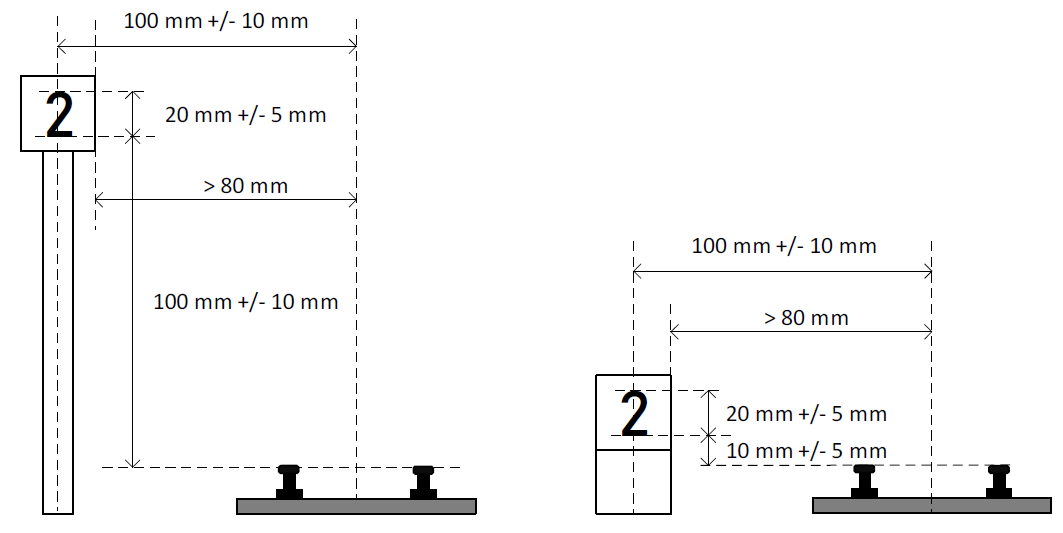
\includegraphics[width=0.8\textwidth]{Signal.png}
        \caption{Auszug aus der Aufgabenstellung: Signaltafel}
    \end{figure}

    Um das Problem «Signalerkennung» zu lösen gibt es eine reine Informatik- Lösung oder eine kombinierte
    Lösung Elektrotechnik - Informatik. \\

    \textbf{Informatik: }
    Bei der Informatiklösung setzt man auf eine Objekterkennung mittels Kamera. Die Kamera nimmt während der Fahrt
    kontinuierlich auf und erkennt wenn ein Signal auftaucht. Anschliessend nimmt die Kamera ein Foto der Tafel auf und
    analysiert die aufgedruckte Zahl. 

    \begin{flushleft}
        \begin{table}[H]
        \begin{tabular}{ | l | p{11cm} |}
        \hline
        \textbf{Problemstellung} & Signalerkennung \\ \hline
        \textbf{Disziplin} & Informatik \\ \hline
        \textbf{Lösungskonzept} & Erkennung mittels Kamera \\ \hline
        \textbf{Komponente} & OV5647 \\ \hline
        \textbf{Bewertung} &  \begin{itemize}
                                \item[+] Einfachheit (Hardware)
                                \item[+] kostengünstig
                                \item[-] Schnelligkeit
                                \item[-] Komplexität (Software)   
                              \end{itemize} \\ \hline
        \end{tabular}
        \caption{Konzeptbeurteilung: Signalerkennung mittels Kamera}
        \label{tab:konzept_wurfel_Stereokamera}
    \end{table}
    \end{flushleft}

    \textbf{Elektrotechnik - Informatik: }
    Bei der kombinierten Lösung wird das Gesamtproblem in ihre Teilprobleme aufgeteilt und jedes Teilproblem
    individuell gelöst. Zur Erkennung der Tafel wird der Ultraschallsensor verwendet. Dieser an der Seite des Zuges
    angebrachte Sensor detektiert die Tafel und sendet ein Signal zur Kamera. Die Kamera nimmt dann ein Bild von der Tafel
    auf und analysiert die Zahl.\\

    \begin{figure}[H]
        \centering
        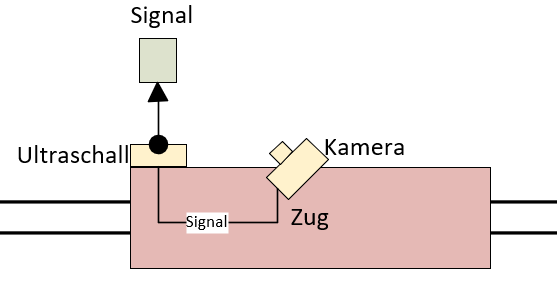
\includegraphics[width=0.7\textwidth]{signal_kombi.png}
        \caption{Signalerkennung mittels Ultraschallsensor und Kamera}
    \end{figure}

    \vspace{1cm}
    \begin{flushleft}
        \begin{table}[H]
        \begin{tabular}{ | l | p{11cm} |}
        \hline
        \textbf{Problemstellung} & Signalerkennung \\ \hline
        \textbf{Disziplin} & Elektrotechnik - Informatik \\ \hline
        \textbf{Lösungskonzept} & Erkennung mittels Ultraschallsensor und Kamera \\ \hline
        \textbf{Komponente} & HC-SR04 / OV5647 \\ \hline
        \textbf{Bewertung} &  \begin{itemize}
                                \item[+] Schnelligkeit
                                \item[+] Einfachheit
                                \item[-] Zuverlässigkeit
                                \item[-] Aufwand (Hardware)   
                              \end{itemize} \\ \hline
        \end{tabular}
        \caption{Konzeptbeurteilung: Signalerkennung mittels Ultraschallsensor und Kamera}
        \label{tab:konzept_wurfel_Stereokamera}
    \end{table}
    \end{flushleft}
\end{document}
